In the beginning and the end of the genetics accelerator pipeline lies the rated and the unrated pools, respectively.
The rated and unrated pools are caches of genetics individuals that waiting to either 1) get selected and be sent through the pipeline, 2) die, or 3) get picked up by a fitness core for fitness ranking.
The rated pool contains individuals stored with a fitness score, and are the indivuiduals that have just been inserted into the accelerator by a fitness core.
The unrated pool contains individuals that have no fitness score calculated.
They are the new individuals produced by the accelerator pipeline, and are waiting to be picked up and rated by a fitness core.

The rated and unrated pools are implemented in \gls{BRAM} on the FPGA for as fast access times as possible.
This is essential to achieve a high memory throughput when executing the algorithms.

It is important to note that the two pools are designed as separate \gls{BRAM} devices.
This is done to achieve even better memory throughput.
The increased throughput is achieved because the different computational units can work on the rated and unrated pools simultaneously.
For instance while one fitness core is storing a ranked individual, another fitness core may be fetching a new individual for ranking. 

Access to the \gls{rated pool} and the \gls{unrated pool} is managed by control units referred to as the \gls{rated controller} and the \gls{unrated controller}.
As with the \gls{data controller} for data memory access, these controllers are responsible for granting access to the rated and unrated pools.
As shown in figure \vref{fpga:fig:genetic:genetic_pipeline}, the genetics accelerator has its own data buses connected to the fitness cores separate from the data bus that is connected to the regular shared data memory, to increase performance by reducing bus conflicts.

The controllers are based on the same principles as the \gls{data controller} described in section \vref{subsec:fpga-data-memory}.
When in need of performing genetic operations, the fitness cores need to request the data bus by setting some request signals.
The combination of these signals refer to the operation the fitness core requests from the genetic controller. 

The controllers continuously perform simple round-robin request handling schemes in order to grant bus access to the next requesting fitness cores, and to the genetic pipeline.
The logic for the \gls{rated controller} is implemented as a state machine, while the \gls{unrated controller}'s simple structure allows it not have one at all.

As the timing diagrams in figure \vref{fpga:fig:timing:genetic:rated_genetic_proc} and \vref{fpga:fig:timing:unrated_genetic_proc} show, both controllers are highly optimized for speed. The single occation where the bus is unused is the cycle in which the \ref{genetic controller} tells the \gls{rated controller} that it no longer requires access.

\begin{figure}[H]
  \centering
  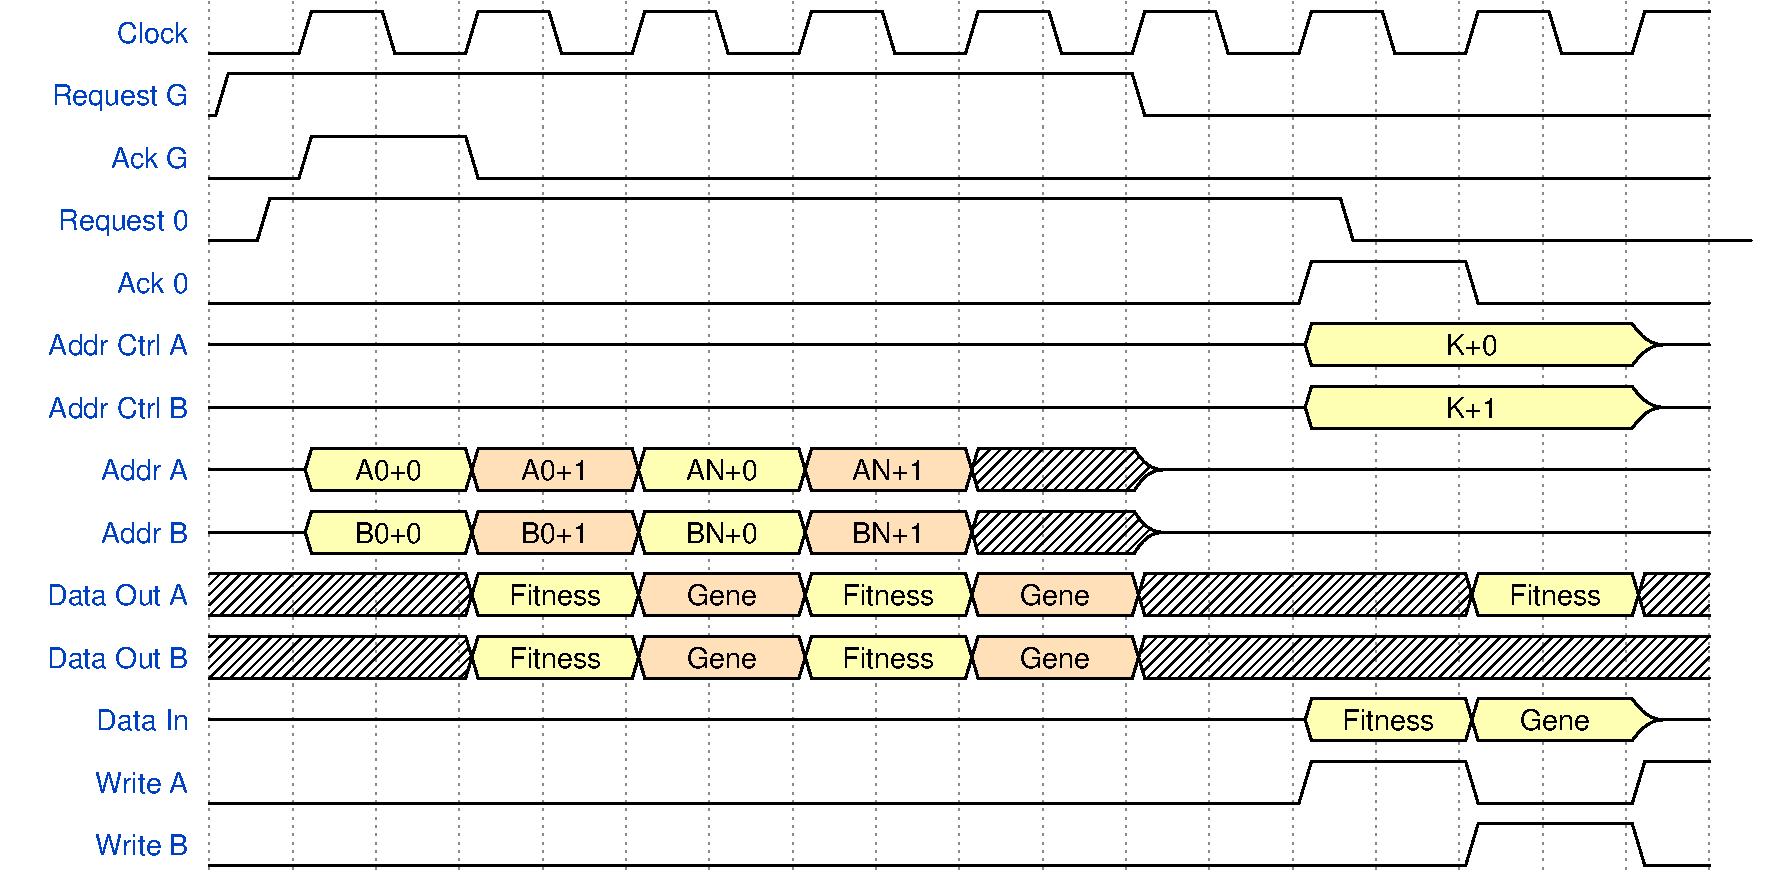
\includegraphics[width=\textwidth]{fpga/fig/timing/rated_genetic_proc.pdf}
  \caption{Fitness values and individuals being read by the selection cores followed by a fitness core writing a new fitness and individual.}
  \label{fpga:fig:timing:genetic:rated_genetic_proc}
\end{figure}

\begin{figure}[H]
  \centering
  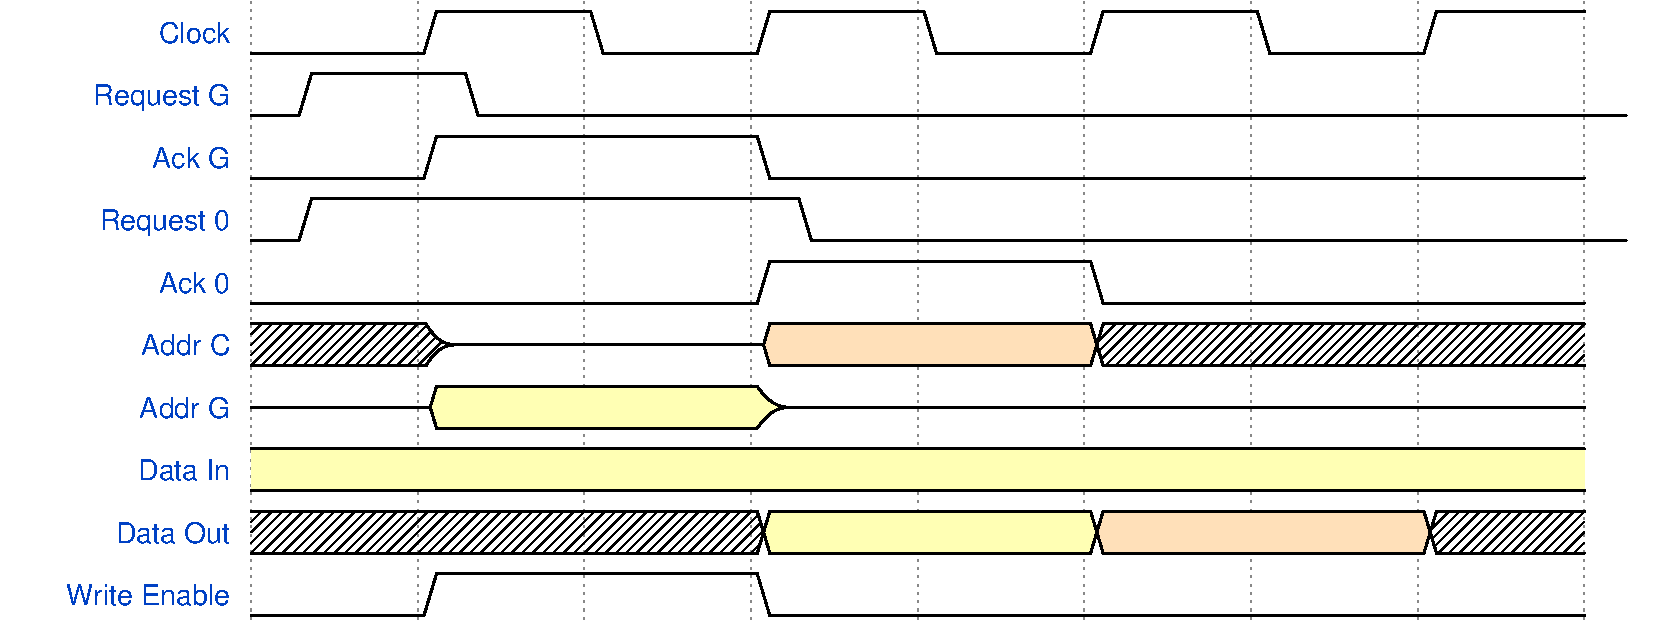
\includegraphics[width=\textwidth]{fpga/fig/timing/unrated_genetic_proc.pdf}
  \caption{A two-induvidual selection core access }
  \label{fpga:fig:timing:genetic:unrated_genetic_proc}
\end{figure}

